\renewcommand{\prevlecture}{7 }
\renewcommand{\thislecture}{8 }
\renewcommand{\nextlecture}{9 }

%
% Cover page
%

\title[PHYS 201 / Lecture \thislecture]
{
  PHYS 201 / Lecture \thislecture\\
  {\it
       Generalizing Maxwell's eqs for time-dependent fields: \\
      Faraday's law and Maxwell's correction to Ampere's law
  }\\
}

\author[C.Andreopoulos] {
  Professor Costas Andreopoulos\inst{1,2}, {\it FHEA}
}
\institute[Liverpool/STFC-RAL] {
   \inst{1} University of Liverpool, Department of Physics\\
   \vspace{0.1cm}
   \inst{2} U.K. Research \& Innovation (UKRI), Science \& Technology Facilities Council,\\
            Rutherford Appleton Laboratory, Particle Physics Department\\
   \vspace{0.5cm}
   {\it {\color{magenta} Lectures delivered at the University of Liverpool, 2020-21}}\\
   \vspace{0.2cm}
}
\date{\today}

\titlegraphic{
  
\includegraphics[height=25px]{./images/logo/liverpool.png}
  \hspace{3px}
  
\includegraphics[height=30px]{./images/logo/ral.png}
}


\begin{frame}[plain]
  \titlepage
\end{frame}

% ------------------------------------------------------------------------------
% ------------------------------------------------------------------------------

%
% Revision of previous lecture
%

\renewcommand{\lecturesummarytitle}{Revision }

\renewcommand{\summarizedlecture}{7 }

%
%
%

\begin{frame}{Lecture \summarizedlecture revision}

In the last lecture:\\

\begin{itemize}

   \item We completed the study of {\bf Maxwell's eqs. in materials (for static fields)}
             and emphasized the analogies between electrostatics and magnetostatics.

   \vspace{0.2cm}

   \item We discussed the magnetic properties of materials
             ({\bf diamagnetism}, {\bf paramagnetism} and {\bf ferromagnetism})
             and developed arguments to understand the physical origins.

   \vspace{0.2cm}

   \item We found out how to {\bf extend Maxwell's eqs. in vacuum}
             in the case of {\bf time-dependent fields}.

\end{itemize}

\end{frame}

%
%
%

\begin{frame}{Lecture \summarizedlecture revision (Magnetic moment / magnetization)}

\begin{columns}
  \begin{column}{0.25\textwidth}
    \begin{center}
      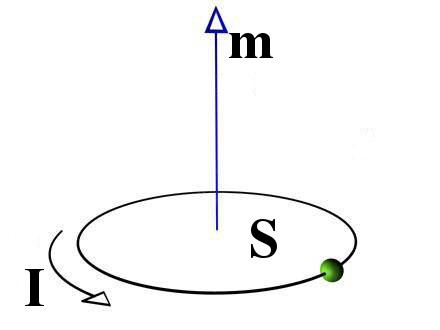
\includegraphics[width=0.95\textwidth]{./images/schematics/magnetic_dipole_moment_00.jpg}\\
    \end{center}
  \end{column}
  \begin{column}{0.70\textwidth}
    We defined the {\bf magnetic dipole moment} $\vec{m}$ as:
   \begin{equation*}
     \vec{m} = I \vec{S}
   \end{equation*}
  \end{column}
\end{columns}

\vspace{0.2cm}

An external magnetic field $\vec{B}$ exerts a torque $\vec{T}$ on a magnetic dipole $\vec{m}$ which is given by:
\begin{equation*}
  \vec{T} = \vec{m} \times \vec{B}
\end{equation*}

This will tend to {\bf align} the previously randomised {\bf magnetic moments}
and {\bf create magnetisation at a macroscopic level}.\\
\vspace{0.2cm}

We define {\bf magnetisation} $\vec{M}$ as the amount of {\bf magnetic dipole moment per unit volume}.

\end{frame}

%
%
%

\begin{frame}{Lecture \summarizedlecture revision (Magnetization-induced currents)}

The {\bf magnetisation induces surface and volume currents}.\\
\vspace{0.3cm}
We can easily be convinced, although we will not show it mathematically,
that the {\bf density of the surface current} is:
\begin{equation*}
  j_{m}^{surf} = \vec{M} \times \hat{n}
\end{equation*}

\vspace{0.1cm}

whereas the {\bf density of the volume current} is:
\begin{equation*}
  j_{m}^{vol} = \vec{\nabla} \times \vec{M}
\end{equation*}

\begin{center}
  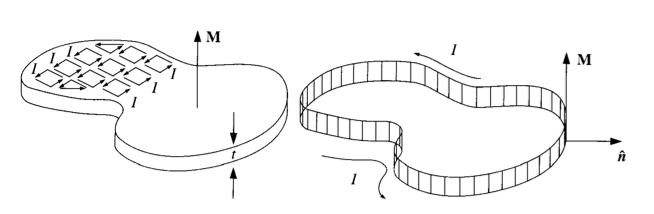
\includegraphics[width=0.98\textwidth]{./images/schematics/magnetization_currents_01.png}\\
\end{center}

\end{frame}

%
%
%

\begin{frame}{Lecture \summarizedlecture revision (Ampere's law in materials)}

We started from Ampere's law in vacuum:
\begin{equation*}
  \vec{\nabla} \times \vec{B} = \mu_0 \vec{j}
\end{equation*}
By writing the total current density $\vec{j}$ as the vector sum of the free ($\vec{j}_{f}$)
and magnetization ($\vec{j}_{m}$) current densities,
and expressing $\vec{j}_{m}$ in terms of the
magnetization field $\vec{M}$ ($\displaystyle \vec{j}_{m} = \vec{\nabla} \times \vec{M}$),
we finally wrote Ampere's law as:
\begin{equation*}
  \vec{\nabla} \times \Big( \frac{\vec{B}}{\mu_0} - \vec{M} \Big) = \vec{j}_{f}
\end{equation*}

We defined the {\bf magnetic field strength} or {\bf magnetic field intensity} $\vec{H}$ as:
\begin{equation*}
  \vec{H} = \frac{\vec{B}}{\mu_0} - \vec{M}
\end{equation*}
In SI, the quantity $\displaystyle \vec{H} = \frac{\vec{B}}{\mu_0} - \vec{M}$ has {\bf units of A/m}.\\

\end{frame}

%
%
%

\begin{frame}{Lecture \summarizedlecture revision (Linear materials)}

Ampere's law in materials is:
$\displaystyle \vec{\nabla} \times \Big( \frac{\vec{B}}{\mu_0} - \vec{M} \Big) = \mu_0 \vec{j}_{f}$\\
\vspace{0.1cm}

If the analogy with electrostatics was exact,
we would write $\vec{M}$ in terms of $\vec{B}$.
However, this is where the analogy breaks.
Instead we typically write:
\begin{equation*}
{\color{magenta}
  \vec{M} = \chi_{m} \vec{H}
}
\end{equation*}
where  $\chi_m$ is the {\bf magnetic susceptibility}.
For {\bf linear materials}, $\chi_m$ is a constant independent of the value of $\vec{H}$.
Expressing $\vec{B}$ in terms of $\vec{H}$:
\begin{equation*}
  \vec{H} = \frac{\vec{B}}{\mu_0} - \vec{M} \Rightarrow
  \vec{B} = \mu_0 \Big( \vec{H} + \vec{M} \Big) \xRightarrow{\vec{M} = \chi_{m} \vec{H}}
  \vec{B} = \Big(1 + \chi_{m} \Big) \mu_0  \vec{H} \Rightarrow
\end{equation*}
\begin{equation*}
  \vec{B} = \mu_r \mu_0 \vec{H} \Rightarrow
  {\color{magenta}
    \vec{B} = \mu \vec{H}
  }
\end{equation*}
where $\mu_r = 1+\chi_{\mu}$
is the {\bf relative permeability} (dimensionless) and
$\mu = \mu_r  \mu_0$ is the {\bf permeability} of the material
(SI unit: $V \cdot s \cdot  A^{-1} \cdot m^{-1}$).\\

\end{frame}

%
%
%

\begin{frame}{Lecture \summarizedlecture revision (Correspondence between quantities)}

{
\setlength{\extrarowheight}{8pt}
\setlength{\arraycolsep}{5pt}

\begin{center}
  \begin{table}[H]
    \begin{tabular}{c|c||c|c}
      \hline
      \multicolumn{2}{c||}{\bf Electrostatics} &
      \multicolumn{2}{c}  {\bf Magnetostatics} \\
      \hline
         {\scriptsize electric dipole moment} &
         $\vec{p} = q \vec{d}$ &
         $\vec{m} = I \vec{S}$ &
         {\scriptsize magnetic dipole moment} \\
      \hline
         {\scriptsize torque within $\vec{E}$ field} &
         $\vec{T} = \vec{p} \times \vec{E}$ &
         $\vec{T} = \vec{m} \times \vec{B}$ &
         {\scriptsize torque within a $\vec{B}$ field} \\
      \hline
         {\scriptsize polarization} &
         $\vec{P}  = \frac{(e.d.m)}{volume}$ &
         $\vec{M} = \frac{(m.d.m)}{volume}$ &
         {\scriptsize magnetization} \\
      \hline
         {\scriptsize surface charge density} &
         $\sigma_{P} = \vec{P} \cdot \hat{n}$ &
         $j_{m}^{surf} = \vec{M} \times \hat{n}$ &
         {\scriptsize surface current density} \\
      \hline
         {\scriptsize volume charge density} &
         $\rho_{P} = - \vec{\nabla} \cdot \vec{P}$ &
         $j_{m}^{vol} = \vec{\nabla} \times \vec{M}$ &
         {\scriptsize volume current density} \\
      \hline
         {\scriptsize electric displacement} &
         $\vec{D} = \epsilon_0 \vec{E} + \vec{P}$ &
         $\vec{H} = \frac{\vec{B}}{\mu_0} - \vec{M}$ &
         {\scriptsize magnetizing field} \\
      \hline
         \multirow{2}{*}{\scriptsize Gauss' law in materials} &
         $\vec{\nabla} \cdot \vec{D} = \rho_{f}$ &
         $\vec{\nabla} \times \vec{H} = \vec{j}_{f}$ &
         \multirow{2}{*}{\scriptsize Ampere's law in materials} \\
      \hhline{~--~}
         &
         $\oint_{S} \vec{D} \cdot d\vec{S} = Q_{f}$ &
         $\oint_{L} \vec{H} \cdot d\vec{\ell} = I_{f}$ &
         \\
      \hline
    \end{tabular}
  \end{table}
\end{center}
}

\end{frame}

%
%
%

\begin{frame}{Lecture \summarizedlecture revision (Magnetic properties of materials)}

\begin{itemize}

\item We also discussed the {\bf magnetic properties of materials}
          and developed (classical) arguments to understand the {\bf physical origins}.

\item The material which has the {\bf most striking and well known
          magnetic properties is iron (Fe).}

     \begin{itemize}
            \item Nickel (Ni), Cobalt (Co), Gadolinium (Gd) and Dysprosium (Dy) behave similarly.
                      We call these materials {\bf \color{magenta} ferromagnets}.
            \item Not only these materials can have a significant magnetisation when inside an
                      external magnetic field, they also {\bf retain their magnetisation in the absence
                      of an external magnetic field.}
     \end{itemize}

\item But {\bf other substances get magnetised too} (water, wood, frogs,...)

     \begin{itemize}
             \item The magnetic effects for these materials are {\bf very very weak!}
             \item Moreover, water, wood, and frogs {\bf do not remain magnetized} once the external
                       magnetic field is removed.
             \item In a presense of an external magnetic field these substances can be magnetised
                       either in the direction of the field ({\color{magenta} {\bf paramagnetic}} substances),
                       or opposite to it ({\color{magenta} {\bf diamagnetic}} substances).
     \end{itemize}

\end{itemize}

\end{frame}

%
%
%

\begin{frame}{Lecture \summarizedlecture revision (Maxwell's eqs. for the static case)}

{\small

\begin{center}
{
  \begin{table}[H]
    \begin{tabular}{|l|c|c|}
      \hline
        \multicolumn{3}{|l|} {
          {\color{magenta}
           {\bf Static case in vacuum}
          }
        }\\
      \hline
      {\bf Gauss's law} &
        $\displaystyle \oint \vec{E} \cdot d\vec{S} = \frac{1}{\epsilon_0} \int \rho d\tau$ &
        $\displaystyle \vec{\nabla} \cdot \vec{E} = \frac{\rho}{\epsilon_0}$ \\

      {\bf Circuital law} &
        $\displaystyle \oint \vec{E} \cdot d\vec{\ell} = 0$ &
        $\displaystyle \vec{\nabla} \times \vec{E} = 0$ \\

      {\bf Gauss's law} (magn.) &
        $\displaystyle \oint \vec{B} \cdot d\vec{S} = 0$ &
        $\displaystyle \vec{\nabla} \cdot \vec{B} = 0$ \\

      {\bf Ampere's law} &
        $\displaystyle \oint \vec{B} \cdot d\vec{\ell} = \mu_{0} \int \vec{j} \cdot d\vec{S}$ &
        $\displaystyle \vec{\nabla} \times \vec{B} = \mu_{0} \vec{j}$ \\

      \hline
    \end{tabular}
  \end{table}
}
\end{center}

\begin{center}
{
  \begin{table}[H]
    \begin{tabular}{|l|c|c|}
      \hline
        \multicolumn{3}{|l|} {
          {\color{magenta}
           {\bf Static case within materials}
          }
        }\\
      \hline
      {\bf Gauss's law} &
        $\displaystyle \oint \vec{D} \cdot d\vec{S} =  \int \rho_{f} d\tau$ &
        $\displaystyle \vec{\nabla} \cdot \vec{D} = \rho_{f}$ \\

      {\bf Circuital law} &
        $\displaystyle \oint \vec{E} \cdot d\vec{\ell} = 0$ &
        $\displaystyle \vec{\nabla} \times \vec{E} = 0$ \\

      {\bf Gauss's law} (magn.) &
        $\displaystyle \oint \vec{B} \cdot d\vec{S} = 0$ &
        $\displaystyle \vec{\nabla} \cdot \vec{B} = 0$ \\

      {\bf Ampere's law} &
        $\displaystyle \oint \vec{H} \cdot d\vec{\ell} =  \int \vec{j}_{f} \cdot d\vec{S}$ &
        $\displaystyle \vec{\nabla} \times \vec{H} = \vec{j}_{f}$ \\
      \hline
    \end{tabular}
  \end{table}
}
\end{center}
}

\end{frame}


%
% Plan for this lecture
%

\begin{frame}{Plan for Lecture \thislecture}

In this lecture:
\begin{itemize}
   \item We will study how we need to {\bf extend Maxwell's eqs. in vaccum}
         in the case of {\bf time-dependent fields}.
\end{itemize}

\end{frame}

% ------------------------------------------------------------------------------
% ------------------------------------------------------------------------------

%
%
%

\begin{frame}{Time-dependent fields}

Having completed the study of Maxwell's equations for the static case (both in vaccum and in materials),
we will now turn our attention to the case where the electric and magnetic field can vary with time.

\begin{center}
   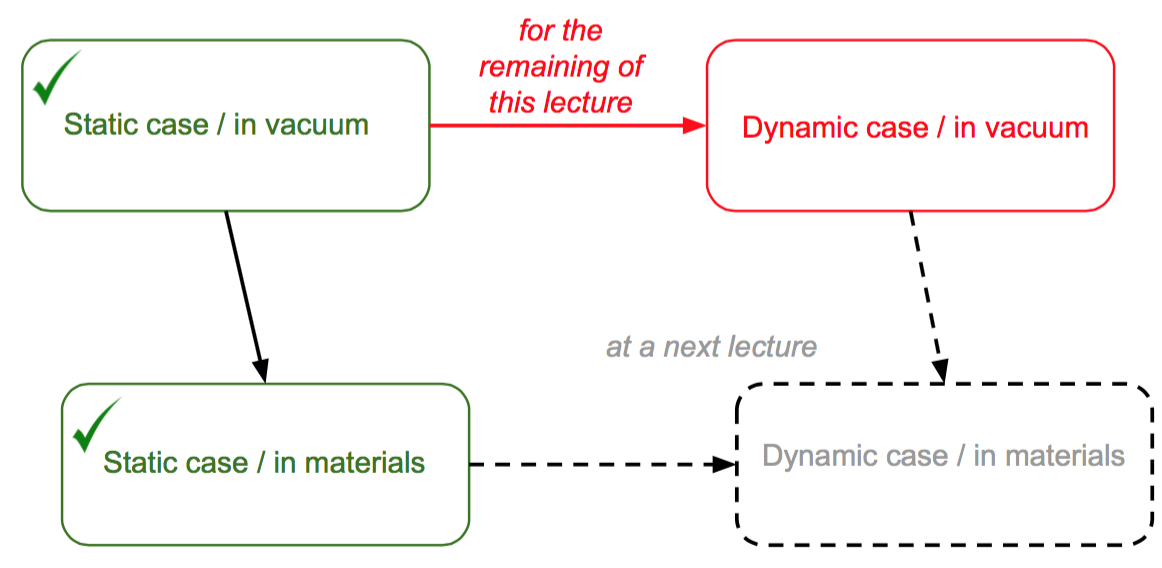
\includegraphics[width=0.95\textwidth]{./images/schematics/maxwell_eq_variations.png}\\
\end{center}

\end{frame}

%
%
%

\begin{frame}{A conductor moving in a magnetic field}

Consider a conductor with length L moves with velocity $\vec{u}$ inside a
homogenous magnetic field $\vec{B}$, as shown below:

\begin{center}
  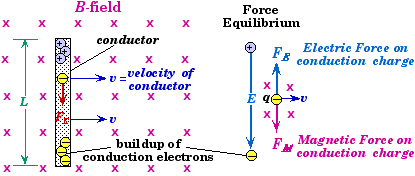
\includegraphics[width=0.60\textwidth]{./images/schematics/conductor_in_magnetic_field_induced_emf.png}\\
\end{center}

\vspace{0.1cm}
Each electron in the conductor feels a magnetic force $\vec{F}_{M} = q \vec{u} \times \vec{B}$.\\
\vspace{0.1cm}
That magnetic force {\bf induces the build-up of charge}
which {\bf produces an electric field} $\vec{E}$:
Each electron feels an electric force $\vec{F}_{E} = q \vec{E}$.\\
\vspace{0.2cm}
The resulting {\bf electric force} $\vec{F}_{E}$ {\bf opposes the magnetic force} $\vec{F}_{M}$.

\end{frame}

%
%
%

\begin{frame}{A conductor moving in a magnetic field}

\begin{columns}
  \begin{column}{0.45\textwidth}
    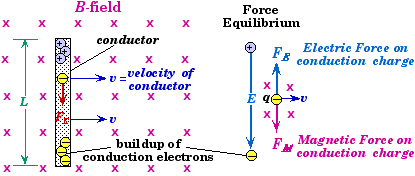
\includegraphics[width=0.98\textwidth]{./images/schematics/conductor_in_magnetic_field_induced_emf.png}\\
  \end{column}
  \begin{column}{0.55\textwidth}
    At equilibrium, the electric and magnetic forces are equal in strength:
    \begin{equation*}
      \vec{F}_{E} =  \vec{F}_{M} \Rightarrow
       \cancel{q} \vec{E} = \cancel{q} \vec{u} \times \vec{B} \Rightarrow
     \end{equation*}
     \begin{equation*}
       \vec{E} = \vec{u} \times \vec{B}
     \end{equation*}
  \end{column}
\end{columns}

\vspace{0.4cm}

An electrical potential difference develops between the ends of the moving conductor,
which becomes a source of EMF:
\begin{equation*}
   \mathcal{E} = \int_{L} \vec{E} \cdot d\vec{\ell} = \int_{L} \Big( \vec{u} \times \vec{B} \Big) \cdot d\vec{\ell}
\end{equation*}

For a closed circuit:
\begin{equation*}
   \mathcal{E} = \oint_{L} \vec{E} \cdot d\vec{\ell} = \oint_{L} \Big( \vec{u} \times \vec{B} \Big) \cdot d\vec{\ell}
\end{equation*}

\end{frame}


%
%
%

\begin{frame}{A circuit moving through a magnetic field}

Now let's consider a simple rectangular circuit moving through a region that has a magnetic field $\vec{B}$:
\begin{center}
  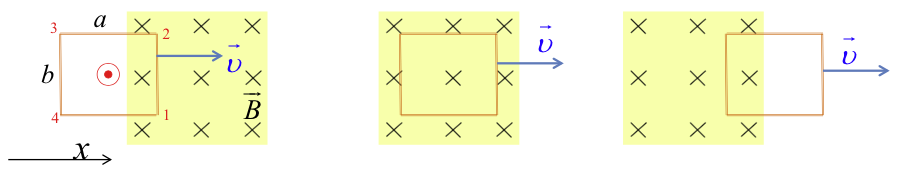
\includegraphics[width=0.98\textwidth]{./images/schematics/circuit_moving_through_magnetic_field_all_3.png}\\
\end{center}

Conventions:
\begin{itemize}
  \item $\vec{B}$ is towards the page.
  \item Assuming current I flows anti-clockwise.
  \item Looping within the circuit: anti-clockwise
  \item Following the direction of the current I with our right-hand, the thumb points towards you -
        let's use that direction for the surface vector
\end{itemize}

\end{frame}

%
%
%

\begin{frame}{A circuit moving through a magnetic field}

\begin{columns}
  \begin{column}{0.30\textwidth}
    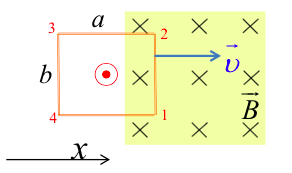
\includegraphics[width=0.99\textwidth]{./images/schematics/circuit_moving_through_magnetic_field_left.png}\\
  \end{column}
  \begin{column}{0.70\textwidth}
    Let's consider what happens as the circuit enters in the region of the magnetic field.
  \end{column}
\end{columns}

\vspace{0.3cm}

\begin{columns}[t]
  \begin{column}{0.50\textwidth}
  {\scriptsize
    \underline{EMF}:\\
    \vspace{0.1cm}
    \begin{itemize}
       \item Side `12':
             $\mathcal{E} = \int \Big( \vec{u} \times \vec{B} \Big) \cdot d\vec{\ell} = uBb$
       \item Side `34' ($\vec{B}=0$):
             $\mathcal{E} = 0$
       \item Side `23' and `14' ($\vec{u} \times \vec{B}$ $\perp$ $d\vec{\ell}$):
             $\mathcal{E} = 0$
       \item Summing-up the EMFs for all 4 sides:
            {\color{magenta}
              \begin{equation*}
               \mathcal{E} = \oint \vec{E} \cdot d\vec{\ell} = uBb
              \end{equation*}
            }
    \end{itemize}
  }
  \end{column}
  \begin{column}{0.50\textwidth}
  {\scriptsize
    \underline{Change in flux}:\\
    \begin{equation*}
      \frac{d\Phi_{M}}{dt} =
        \frac{d}{dt} \Big( \int \vec{B} \cdot d\vec{S} \Big) =
        \frac{d}{dt} \Big( \vec{B} \cdot \int d\vec{S} \Big) =
    \end{equation*}
    \begin{equation*}
          \frac{d}{dt} \Big( \vec{B} \cdot \vec{S} \Big) \xlongequal{\angle(\vec{B}, \vec{S}) = \pi}
          \frac{d}{dt} \Big( -BS \Big) \xlongequal{S=bx}
    \end{equation*}
    \begin{equation*}
        \frac{d}{dt} \Big( -Bbx \Big) =
        - \frac{dx}{dt} B b \Rightarrow
    \end{equation*}
    \begin{equation*}
        {\color{magenta}
          \frac{d\Phi_{M}}{dt} = -uBb
        }
    \end{equation*}
  }
  \end{column}
\end{columns}

\end{frame}

%
%
%

\begin{frame}{A circuit moving through a magnetic field}

\begin{columns}
  \begin{column}{0.30\textwidth}
    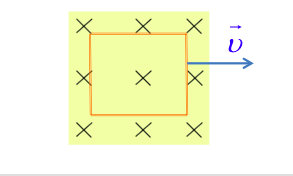
\includegraphics[width=0.99\textwidth]{./images/schematics/circuit_moving_through_magnetic_field_centre.png}\\
  \end{column}
  \begin{column}{0.70\textwidth}
    Let's consider what happens when the circuit is entirely within the region of the magnetic field.
  \end{column}
\end{columns}

\vspace{0.1cm}

\begin{columns}[t]
  \begin{column}{0.50\textwidth}
  {\scriptsize
    \underline{EMF}:\\
    \vspace{0.2cm}
    \begin{itemize}
       \item Side `12':
             $\mathcal{E} = \int \Big( \vec{u} \times \vec{B} \Big) \cdot d\vec{\ell} = uBb$
       \item Side `34':
             $\mathcal{E} = \int \Big( \vec{u} \times \vec{B} \Big) \cdot d\vec{\ell} = -uBb$\\
             (since $\vec{u} \times \vec{B}$ is same as for side `12',
             but $d\vec{\ell}$ has opposite direction).
       \item Side `23' and `14' ($\vec{u} \times \vec{B}$ $\perp$ $d\vec{\ell}$):
             $\mathcal{E} = 0$
       \item Summing-up the EMFs for all 4 sides:
            {\color{magenta}
              \begin{equation*}
               \mathcal{E} = \oint \vec{E} \cdot d\vec{\ell} = 0
              \end{equation*}
            }
    \end{itemize}
  }
  \end{column}
  \begin{column}{0.50\textwidth}
  {\scriptsize
    \underline{Change in flux}:\\
    \vspace{0.1cm}
    The circuit is entirely within the magnetic field so, as it moves,
    there are as many magnetic field line entering its surface as ones exiting.
    The rate of change of the magnetic flux is 0.
    {\color{magenta}
      \begin{equation*}
        \frac{d\Phi_{M}}{dt} = 0
      \end{equation*}
    }
  }
  \end{column}
\end{columns}

\end{frame}

%
%
%

\begin{frame}{A circuit moving through a magnetic field}

\begin{columns}
  \begin{column}{0.30\textwidth}
    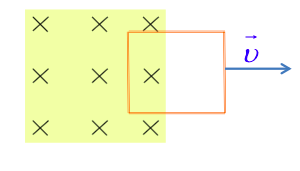
\includegraphics[width=0.99\textwidth]{./images/schematics/circuit_moving_through_magnetic_field_right.png}\\
  \end{column}
  \begin{column}{0.70\textwidth}
    Finally, let's consider what happens as the circuit exits the region of the magnetic field.
  \end{column}
\end{columns}

\vspace{0.3cm}

\begin{columns}[t]
  \begin{column}{0.50\textwidth}
  {\scriptsize
    \underline{EMF}:\\
    \vspace{0.1cm}
    \begin{itemize}
       \item Side `12' ($\vec{B}=0$):
             $\mathcal{E} = 0$
       \item Side `34':
             $\mathcal{E} = \int \Big( \vec{u} \times \vec{B} \Big) \cdot d\vec{\ell} = -uBb$
       \item Side `23' and `14' ($\vec{u} \times \vec{B}$ $\perp$ $d\vec{\ell}$):
             $\mathcal{E} = 0$
       \item Summing-up the EMFs for all 4 sides:
            {\color{magenta}
              \begin{equation*}
               \mathcal{E} = \oint \vec{E} \cdot d\vec{\ell} = -uBb
              \end{equation*}
            }
    \end{itemize}
  }
  \end{column}
  \begin{column}{0.50\textwidth}
  {\scriptsize
    \underline{Change in flux}:\\
    \begin{equation*}
      \frac{d\Phi_{M}}{dt} =
        \frac{d}{dt} \Big( \int \vec{B} \cdot d\vec{S} \Big) =
        \frac{d}{dt} \Big( \vec{B} \cdot \int d\vec{S} \Big) =
    \end{equation*}
    \begin{equation*}
          \frac{d}{dt} \Big( \vec{B} \cdot \vec{S} \Big) \xlongequal{\angle(\vec{B}, \vec{S}) = \pi}
          \frac{d}{dt} \Big( -BS \Big) \xlongequal{S=bx}
    \end{equation*}
    \begin{equation*}
        \frac{d}{dt} \Big( -Bbx \Big) =
        - \frac{dx}{dt} B b = -(-u) B b \Rightarrow
    \end{equation*}
    \begin{equation*}
        {\color{magenta}
          \frac{d\Phi_{M}}{dt} = uBb
        }
    \end{equation*}
  }
  \end{column}
\end{columns}

\end{frame}

%
%
%

\begin{frame}{A circuit moving through a magnetic field}

A rectangular circuit moving through a region with magnetic field $\vec{B}$:
\begin{center}
  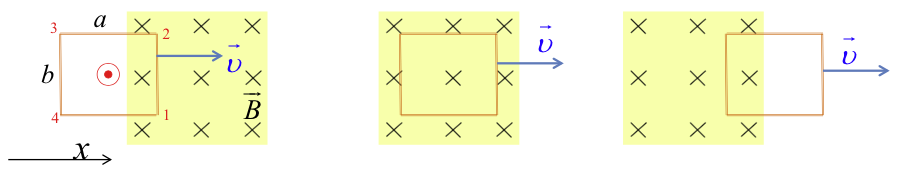
\includegraphics[width=0.88\textwidth]{./images/schematics/circuit_moving_through_magnetic_field_all_3.png}
\end{center}

\begin{columns}
  \begin{column}{0.55\textwidth}
  In summary:
  {\small
    \setlength{\extrarowheight}{10pt}
    \setlength{\arraycolsep}{5pt}
    \begin{table}[H]
        \begin{tabular}{|c||c|c|}
        \hline
               & $\displaystyle \oint_{L} \vec{E} \cdot d\vec{\ell}$ & $\displaystyle \frac{d\Phi_{M}}{dt}$\\
        \hline
          left   &  uBb &  -uBb \\
          centre & 0    &  0   \\
          right  &  -uBb & uBb \\
        \hline
        \end{tabular}
    \end{table}
  }
  \end{column}
  \begin{column}{0.45\textwidth}
     So, indeed, in all cases:
     \begin{equation*}
       \mathcal{E} = \oint_{L} \vec{E} \cdot d\vec{\ell} = - \frac{d\Phi_{M}}{dt}
     \end{equation*}
  \end{column}
\end{columns}

\end{frame}

%
%
%

\begin{frame}{Faraday's observations}

In 1831 Michael Faraday reported on a series of experiments.\\
\vspace{0.2cm}

A current flows in a wire loop when:
\vspace{0.2cm}
\begin{enumerate}[(a)]
{\small
  \item the loop is pulled through a magnetic field,
  \item the loop is at rest but the magnet moves in the opposite direction, and
  \item both the loop and the magnet are at rest but the strength of the magnetic field is varied
}
\end{enumerate}

\begin{center}
  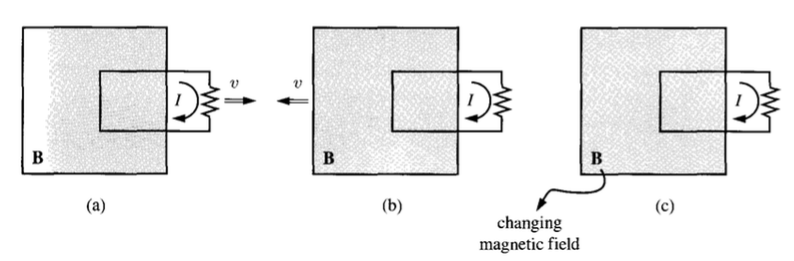
\includegraphics[width=0.88\textwidth]{./images/schematics/faraday_law_schematic.png}
\end{center}

\end{frame}


%
%
%

\begin{frame}{Faraday's observations}

\begin{center}
  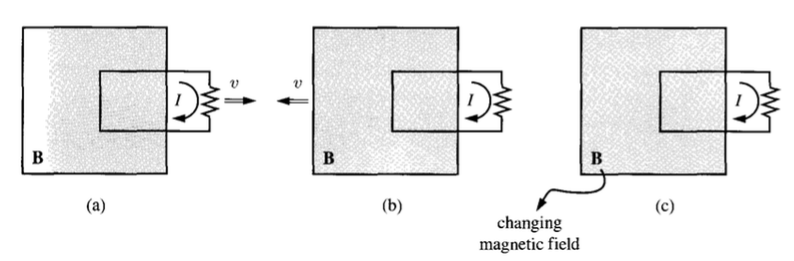
\includegraphics[width=0.88\textwidth]{./images/schematics/faraday_law_schematic.png}\\
\end{center}

\begin{itemize}
   \item In cases (a) and (b) it is the {\bf magnetic field} that is {\bf responsible for the EMF}
             (as in the example we studied earlier).
    \item But in case (c) both the loop and the magnet are stationary and the force felt
              by the electrons can not be magnetic.
              It is the {\bf electric field} that is {\bf responsible for the EMF}!
\end{itemize}

This led Faraday to realize that:
\begin{center}
{\bf A time-varying magnetic field induces an electric field}
\end{center}

\end{frame}

%
%
%

\begin{frame}{Faraday's law / Lenz's law}

In all cases the {\bf motional EMF} is directly related
to the {\bf change of the magnetic flux $\Phi_{M}$ though the circuit}:\\

\vspace{0.1cm}

\begin{columns} [T]
  \begin{column}{0.25\textwidth}
    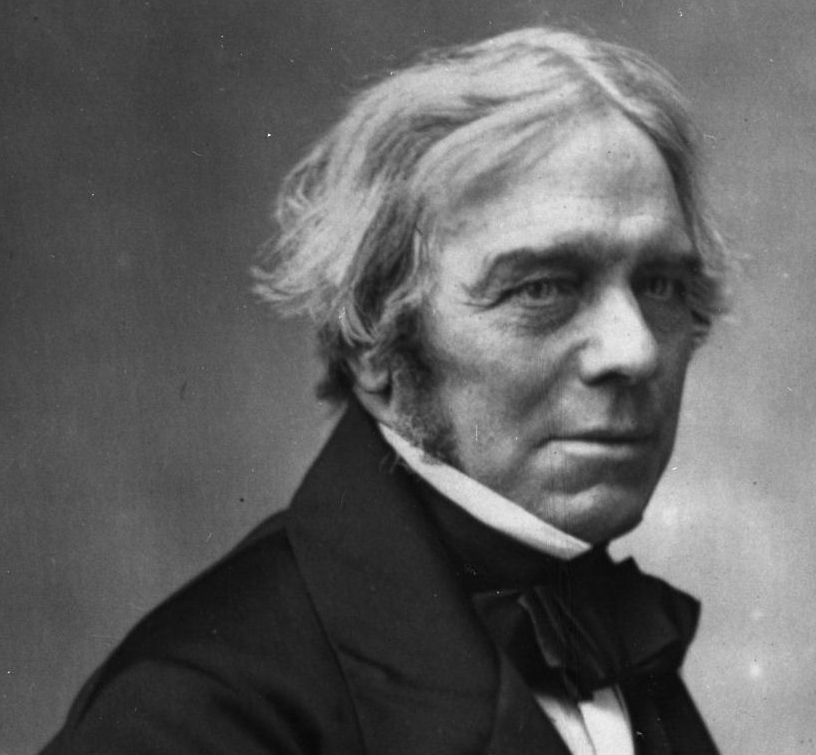
\includegraphics[width=0.98\textwidth]{./images/people/faraday.png}\\
    {\tiny Michael Faraday (1791 - 1867).}
  \end{column}
  \begin{column}{0.75\textwidth}
   \begin{center}
    {\color{red}
    \begin{equation*}
      \mathcal{E} = \oint_{L} \vec{E} \cdot d\vec{\ell} = - \frac{d\Phi_{M}}{dt}
    \end{equation*}
    }
    \vspace{0.2cm}
    This is the so-called {\bf Faraday's law} (integral form).
   \end{center}
  \end{column}
\end{columns}

\vspace{0.1cm}

\begin{columns}
  \begin{column}{0.75\textwidth}
  {\scriptsize
    Lenz' law (1845): The EMF induced by a changing flux has a polarity
    such that the current flowing gives rise to a flux which opposes the change of flux.\\
    \vspace{0.1cm}
    The minus sign is a consequence of the {\bf conservation of energy} and
    of {\bf Newton's 3rd law} of motion: Induction is a an ``inertial reaction''.
    The system develops a current which tries to maintain the flux constant.\\
  }
  \end{column}
  \begin{column}{0.25\textwidth}
    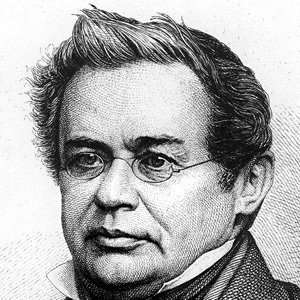
\includegraphics[width=0.83\textwidth]{./images/people/lenz.jpg}\\
    {\tiny Heinrich Lenz (1804 - 1865).}
  \end{column}
\end{columns}

\end{frame}



%
%
%

\begin{frame}{Differential form of Faraday's law}

The integral form of Faraday's law is:
\begin{equation*}
   \oint_{L} \vec{E} \cdot d\vec{\ell} = - \frac{d}{dt} \int_{S} \vec{B} \cdot d\vec{S}
\end{equation*}

Using Stoke's theorem, we obtain its differential form:
\begin{equation*}
   \oint_{L} \vec{E} \cdot d\vec{\ell} = - \frac{d}{dt} \int_{S(L)} \vec{B} \cdot d\vec{S} \Rightarrow
   \int_{S(L)} \Big( \vec{\nabla} \times \vec{E} \Big) \cdot d\vec{S} =
     - \int_{S(L)} \frac{\partial \vec{B}}{\partial t} \cdot d\vec{S} \Rightarrow
\end{equation*}
\begin{equation*}
   \int_{S(L)} \Big( \vec{\nabla} \times \vec{E} + \frac{\partial \vec{B}}{\partial t} \Big) \cdot d\vec{S} = 0  \Rightarrow
   \vec{\nabla} \times \vec{E} + \frac{\partial \vec{B}}{\partial t} = 0 \Rightarrow
\end{equation*}
\begin{equation*}
{\color{red}
   \vec{\nabla} \times \vec{E} = - \frac{\partial \vec{B}}{\partial t}
}
\end{equation*}

\end{frame}



%
% Worked example
%

{
\problemslide

%
%
%

\begin{frame}{Worked example }

\begin{blockexmplque}{Question}
A circular wire loop on the x-y plane has a radius $r_0$ = 1 cm at time t = 0. \\
A homogeneous magnetic field of $3 \times 10^{-3}$ T in the positive z direction permeates the loop.
\begin{enumerate}
  \item Find the magnetic flux through the loop at t=0.
  \item The radius of the loop increases with $\displaystyle r(t) = r_0 + u \cdot t$
        with u = 1 cm/s. Find the magnetic flux through the loop at t = 4 s.
  \item Derive an expression for the EMF in the loop as a function of time.
\end{enumerate}
\end{blockexmplque}

\vspace{0.1cm}


The flux through the loop is given by  $\displaystyle \Phi = \int \vec{B} \cdot d\vec{S}$.

The loop is lying on the x-y plane, hence the surface vector
$d\vec{S}$ that is normal to the loop surface is along the z axis.
$\vec{B}$ is also along the z axis.

Therefore, the above dot product simplifies to $\displaystyle \Phi = \int B dS$.

\end{frame}

%
%
%

\begin{frame}{Worked example }

Since $\vec{B}$ is homogeneous:
\begin{equation*}
     \Phi = B \int  dS =  B \Big( \pi r^2\Big)
\end{equation*}
where $r$ is the radius of the loop.

\vspace{0.4cm}

In our case, r and hence $\Phi$ are functions of time:
\begin{equation*}
     \Phi(t) = B \Big( \pi r(t)^2\Big)
\end{equation*}

\vspace{0.3cm}

At time t = 0:
\begin{equation*}
   \Phi(t = 0) = B \Big( \pi r_0^2 \Big)
      = \Big( 3 \times 10^{-3} \; T \Big) \Big( 3.14  \cdot 0.01^2 \; m^2 \Big) = 9.4 \times 10^{-7} \; T \cdot m^2
\end{equation*}

\end{frame}

%
%
%

\begin{frame}{Worked example }

The radius of the loop increases as $\displaystyle r(t) = r_0 + u \cdot t$,
with u = 1 cm/s.

\vspace{0.3cm}

At t = 4 s, the radius of the loop is:
\begin{equation*}
     r(t = 4 \; s) = 0.01 \; cm + \Big(0.01 \; m/s \Big) \cdot \Big( 4 \; s \Big) = 0.05 \; m
\end{equation*}

\vspace{0.2cm}

Therefore the flux through the loop is now:
\begin{equation*}
     \Phi(4 \; s) = \Big( 3 \times 10^{-3} \; T \Big) \Big( 3.14  \cdot 0.05^2 \; m^2 \Big) = 2.35 \times 10^{-5} \; T \cdot m^2
\end{equation*}

\end{frame}

%
%
%

\begin{frame}{Worked example }

According to Faraday's law, the EMF $\displaystyle \mathcal{E} = \oint \vec{E} d\vec{\ell}$ developed in the wire loop
is equal to the negative rate of change of the magnetic flux through the loop:
\begin{equation*}
      \mathcal{E} = - \frac{d\Phi(t)}{dt} = - \frac{d}{dt} \bigg\{ B
      \Big( \pi r(t)^2\Big) \bigg\}  = - \pi B \frac{d}{dt} \bigg\{ r(t)^2 \bigg\}
\end{equation*}

Recall that $\displaystyle  r(t) = r_0 + u \cdot t$, therefore:
\begin{equation*}
      \mathcal{E}
          = - \pi B \frac{d}{dt} \bigg\{  \Big( r_0 + u \cdot t \Big)^2 \bigg\}
          = - \pi B \frac{d}{dt} \bigg\{  r_0^2 + 2 \cdot r_0 \cdot u \cdot t + u^2 \cdot t^2 \bigg\}
\end{equation*}
\begin{equation*}
      = - \pi B \Big(  2 \cdot r_0 \cdot u + 2\cdot u^2 \cdot t \Big)
      = - 2 \pi B u \Big( r_0 + u \cdot t \Big)
      = - 2 \pi B u r(t)
\end{equation*}

\end{frame}


} % Example


%
%
%

\begin{frame}{A problem with Ampere's law}

Consider a current I charging a parallel plate capacitor.\\
\vspace{0.3cm}
\begin{columns}
  \begin{column}{0.30\textwidth}
   \begin{center}
    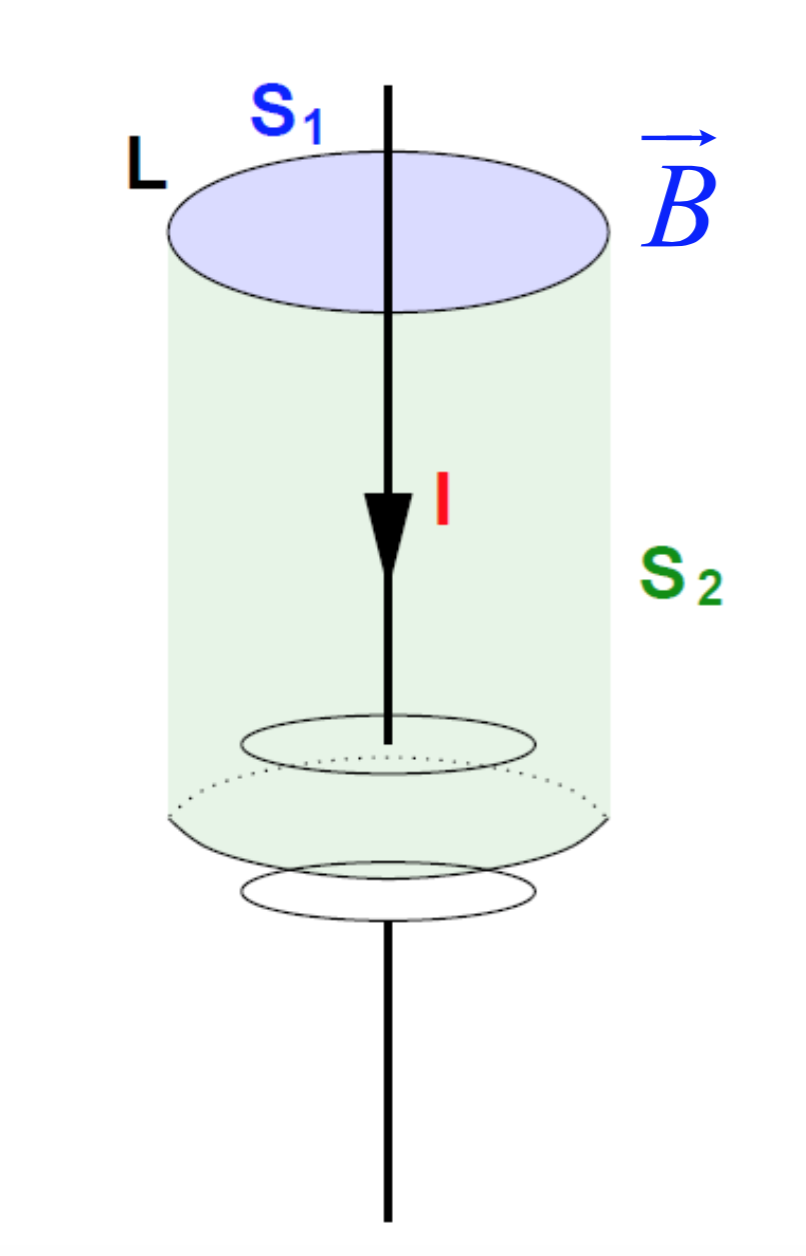
\includegraphics[width=0.95\textwidth]{./images/schematics/problem_with_ampere_law.png}\\
   \end{center}
  \end{column}
  \begin{column}{0.70\textwidth}
  {\small
      Apply Ampere's law for the flat (light blue) surface at the top:
      \begin{equation*}
          \oint_{L} \vec{B} \cdot d\vec{\ell} = \mu_{0} I
     \end{equation*}
     So {\bf there is a magnetic field along L}.\\
     \vspace{0.2cm}
      Now, apply Ampere's law for the ``tophat'' (light green) surface
      made of the cylindrical part (no current flowing through it) and the
      circle between the two conducting plates (also no current):
      \begin{equation*}
          \oint_{L} \vec{B} \cdot d\vec{\ell} = 0
     \end{equation*}
     So {\bf there is NO magnetic field along L}.\\
   }
  \end{column}
\end{columns}

\vspace{0.3cm}

We get {\bf contradictory predictions} for the same path L! What is wrong?

\end{frame}

%
%
%

\begin{frame}{A problem with Ampere's Law}

We get {\bf contradictory predictions} for the same path L! What is wrong?\\
\vspace{0.3cm}

When we studied Faraday's law, we saw that a change in the magnetic field $\vec{B}$
is responsible for creating an electric field $\vec{E}$:
\begin{equation*}
  \vec{\nabla} \times \vec{E} = -\frac{\partial \vec{B}}{\partial t}
\end{equation*}
We should expect that the opposite may be true as well!
A change in the electric field $\vec{E}$ may modify the magnetic field $\vec{B}$.\\

\vspace{0.3cm}

In the example studied previously, the electric field $\vec{E}$ change with time.

\vspace{0.2cm}

How should we extend Ampere's law to take the effects of a changing electric field into account?

\end{frame}

%
%
%

\begin{frame}{Extending Ampere's law}

Let's start from the differential form of Ampere's law:
\begin{equation*}
  \vec{\nabla} \times \vec{B} = \mu_0 \vec{j}
\end{equation*}

We can calculate the divergence of both sides:
\begin{equation*}
  \vec{\nabla} \cdot \Big( \vec{\nabla} \times \vec{B} \Big) = \mu_0 \vec{\nabla} \cdot \vec{j}
\end{equation*}

The left-hand side is 0 (the divergence of the curl of a vector field is always 0).
So the right-hand side has to be 0 as well.
\begin{equation*}
  \vec{\nabla} \vec{j} = 0
\end{equation*}

But this is generally not true!
Recall the continuity equation that expresses the local conservation of charge:
\begin{equation*}
  \vec{\nabla} \cdot \vec{j} = -\frac{\partial \rho}{\partial t}
\end{equation*}

\end{frame}

%
%
%

\begin{frame}{Extending Ampere's law}

Ampere's law, as we know it so far, is at odds with the fundamental principle of
the local conservation of charge. Can we reconcile the two?

The charge density is given by Gauss' law
\begin{equation*}
  \vec{\nabla} \cdot \vec{E} = \frac{\rho}{\epsilon_0} \Rightarrow \rho =
   \epsilon_0 \vec{\nabla} \cdot \vec{E}
\end{equation*}

Taking the partial derivative of $\rho$ with respect to time:
\begin{equation*}
  \frac{\partial \rho}{\partial t} =
   \frac{\partial}{\partial t} \Big( \epsilon_0 \vec{\nabla} \cdot \vec{E} \Big) =
   \vec{\nabla} \cdot \Big( \epsilon_0 \frac{\partial \vec{E}}{\partial t} \Big)
\end{equation*}

Then, the continuity equation:
\begin{equation*}
  \vec{\nabla} \cdot \vec{j} = -\frac{\partial \rho}{\partial t}
\end{equation*}

becomes:
\begin{equation*}
  \vec{\nabla} \cdot \vec{j} =
    - \vec{\nabla} \cdot \Big( \epsilon_0 \frac{\partial \vec{E}}{\partial t} \Big)
\end{equation*}

\end{frame}


%
%
%

\begin{frame}{Extending Ampere's law}

We have written the continuity equation as:
\begin{equation*}
  \vec{\nabla} \cdot \vec{j} = - \vec{\nabla} \cdot \Big( \epsilon_0 \frac{\partial \vec{E}}{\partial t} \Big)
\end{equation*}
which suggests that:
\begin{equation*}
  \vec{\nabla} \cdot \Big( \vec{j} + \epsilon_0 \frac{\partial \vec{E}}{\partial t} \Big) = 0
\end{equation*}

{\bf This is interesting hint!}\\
Maxwell realised that all it takes to fix Ampere's law is to do the following substitution:
\begin{equation*}
  \vec{j} \rightarrow
  \vec{j} + \epsilon_0 \frac{\partial \vec{E}}{\partial t}
\end{equation*}

The term $\displaystyle \epsilon_0 \frac{\partial \vec{E}}{\partial t}$ is called {\bf displacement current}.
\end{frame}

%
%
%

\begin{frame}{Extending Ampere's law}

With this extension (adding the displacement current), Ampere's law is no longer at odds with the
local conservation of charge, as expressed with the continuity equation. Indeed:

\begin{equation*}
  \vec{\nabla} \times \vec{B} =
      \mu_0 \Big( \vec{j} + \epsilon_0 \frac{\partial \vec{E}}{\partial t} \Big)  \Rightarrow
\end{equation*}

\begin{equation*}
  \vec{\nabla} \cdot \Big( \vec{\nabla} \times \vec{B} \Big) =
    \vec{\nabla} \cdot \Big( \mu_0 \vec{j} + \epsilon_0 \mu_0 \frac{\partial \vec{E}}{\partial t} \Big)  \Rightarrow
\end{equation*}

\begin{equation*}
  0 =
    \cancel{\mu_0} \vec{\nabla} \cdot \vec{j} + \epsilon_0 \cancel{\mu_0} \frac{\partial}{\partial t}
    \Big( \vec{\nabla} \cdot  \vec{E}\Big)  \Rightarrow
\end{equation*}

\begin{equation*}
  0 =
    \vec{\nabla} \cdot \vec{j} + \cancel{\epsilon_0} \frac{\partial}{\partial t}
      \Big( \frac{\rho}{\cancel{\epsilon_0}} \Big)  \Rightarrow
\end{equation*}

\begin{equation*}
    \frac{\partial \rho}{\partial t} = - \vec{\nabla} \cdot \vec{j}
\end{equation*}

\end{frame}


%
% Worked example
%

{
\problemslide

%
%
%

\begin{frame}{Worked example }

\begin{blockexmplque}{Question}
\begin{columns}
  \begin{column}{0.22\textwidth}
   \begin{center}
     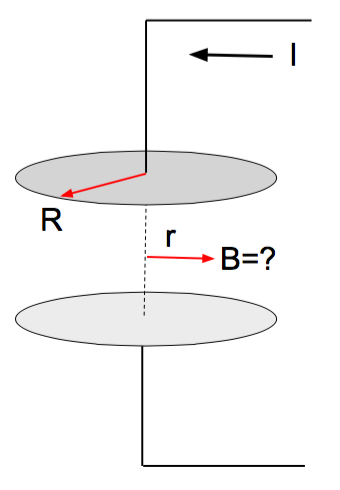
\includegraphics[width=0.90\textwidth]{./images/problems/lect6_capacitor.png}
   \end{center}
  \end{column}
  \begin{column}{0.78\textwidth}
     A parallel-plate capacitor with circular plates of radius R is being
     charged as shown in the figure on the left.\\
     Derive an expression for the magnetic field at radius r (in
     the volume within the two plates) for the case r $\leq$ R.
  \end{column}
\end{columns}
\end{blockexmplque}

\vspace{0.2cm}

A magnetic field can be created either by a current or a changing electric field.
This is expressed by Ampere's law:
\begin{equation*}
    \oint_{L} \vec{B} \cdot d\vec{\ell} = \mu_0 \int_{S} \Big( \vec{j} + \epsilon_0  \frac{\partial \vec{E}}{\partial t} \Big) \cdot d\vec{S}
\end{equation*}

\end{frame}

%
%
%

\begin{frame}{Worked example }

There is no current between the capacitor plates, but the electric flux there is changing.
Thus, Ampere's law reduces to:
\begin{equation*}
    \oint_{L} \vec{B} \cdot d\vec{\ell} = \mu_0 \epsilon_0 \int_{S} \Big( \frac{\partial \vec{E}}{\partial t} \Big) \cdot d\vec{S}
\end{equation*}

\vspace{0.2cm}

We choose a circular Amperian loop with radius r $\le$ R.

\vspace{0.2cm}

The magnetic field $\vec{B}$ at all points along the loop is tangent to the loop, as is the path element $d\vec{\ell}$.
Thus $\vec{B}$ and $d\vec{\ell}$ are parallel or antiparallel at each point of the loop.

\vspace{0.2cm}

For simplicity, assume that we step along the loop in such a way so that $\vec{B}$ and $d\vec{\ell}$ are parallel.
Therefore:
\begin{equation*}
    \oint_{L} \vec{B} \cdot d\vec{\ell} = \oint_{L}  B \; d\ell
\end{equation*}

\end{frame}

%
%
%

\begin{frame}{Worked example }

Due to the circular symmetry of the plates, we can also assume that $\vec{B}$ has the same
magnitude at every point around the loop. Thus, B can be taken outside the integral.

\vspace{0.2cm}

The integral that remains is $\oint_{L}  d\ell$ which simply gives the circumference $2 \pi r$ of the loop.
Therefore, the integral becomes:
\begin{equation*}
    \oint_{L} \vec{B} \cdot d\vec{\ell} = B \; \Big( 2 \pi r\Big)
\end{equation*}

\vspace{0.2cm}

Substituting the above result into Ampere's law gives:
\begin{equation*}
    B \; \Big( 2 \pi r\Big) = \mu_0 \epsilon_0 \int_{S} \Big( \frac{\partial \vec{E}}{\partial t} \Big) \cdot d\vec{S} \Rightarrow
    B = \frac{\mu_0 \epsilon_0}{2 \pi r} \int_{S} \Big( \frac{\partial \vec{E}}{\partial t} \Big) \cdot d\vec{S} \Rightarrow
\end{equation*}
\begin{equation*}
    B = \frac{\mu_0 \epsilon_0}{2 \pi r}  \frac{\partial}{\partial t} \int_{S} \vec{E} \cdot d\vec{S}
\end{equation*}

\end{frame}

%
%
%

\begin{frame}{Worked example }

We assume that the electric field $\vec{E}$ is uniform between the
capacitor plates and directed perpendicular to the plates.
The electric flux through the Amperian loop is simply $EA$,
where $A$ is the (constant) area encircled by the loop within the electric field.
The previous equation becomes:

\begin{equation*}
    B = \frac{\mu_0 \epsilon_0}{2 \pi r}  \frac{d}{dt} \Big( E A \Big)
       = \frac{\mu_0 \epsilon_0}{2 \pi r}  A \frac{dE}{dt}
\end{equation*}

\vspace{0.2cm}

The area A that is encircled by the Amperial loop within the electric field is
the full area $\pi r^2$ of the loop because the loop's radius r is less than (or equal to)
the plate radius R.   Substituting $\pi r^2$ for $A$, we have:
\begin{equation*}
    B = \frac{\mu_0 \epsilon_0}{2 \pi r}  \pi r^2 \frac{dE}{dt} \Rightarrow
    B = \frac{\mu_0 \epsilon_0 r}{2} \frac{dE}{dt}
\end{equation*}

\end{frame}

%
%
%

\begin{frame}{Worked example }

Ignoring edge effects,
the electric field E is uniform within the plates of the parallel plate capacitor
and vanishes outside the volume within the two plates.
Using a cylindrical Gaussian surface whose bases are parallel to the
plates and which encloses the upper plate, we have:
\begin{equation*}
    E \pi R^2 = \frac{Q}{\epsilon_0} \Rightarrow
    E = \frac{1}{\pi R^2 \epsilon_0} Q
\end{equation*}

Therefore, the rate of change of E is given by:
\begin{equation*}
    \frac{dE}{dt} = \frac{1}{\pi R^2 \epsilon_0} \frac{dQ}{dt}
    \xRightarrow {I = dQ/dt}
    \frac{dE}{dt} = \frac{1}{\pi R^2 \epsilon_0} I
\end{equation*}

Substituting the expression for $dE/dt$ in the expression we obtained
earlier for B, we have:
\begin{equation*}
    B = \frac{\mu_0 \epsilon_0 r}{2} \frac{1}{\pi R^2 \epsilon_0} I
    \Rightarrow
    B = \frac{\mu_0 I r}{2 \pi R^2}
\end{equation*}

This is the required expression for the magnetic field at radius r $\le$ R.

\end{frame}



} % end worked example


% ------------------------------------------------------------------------------
% ------------------------------------------------------------------------------

%
% What to remember
%

\renewcommand{\lecturesummarytitle}{Main points to remember }

\renewcommand{\summarizedlecture}{8 }


%
%
%

\begin{frame}{Lecture \summarizedlecture revision (Conductors moving in a magnetic field)}

\begin{columns}
  \begin{column}{0.50\textwidth}
     We consider a conductor with length L moves with velocity $\vec{u}$ inside a
     homogenous magnetic field $\vec{B}$, as shown on the right.
  \end{column}
  \begin{column}{0.50\textwidth}
   \begin{center}
     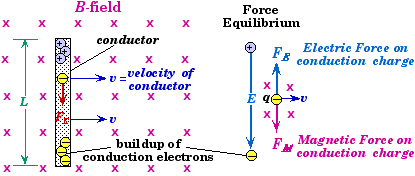
\includegraphics[width=0.90\textwidth]{./images/schematics/conductor_in_magnetic_field_induced_emf.png}\\
   \end{center}
  \end{column}
\end{columns}

\vspace{0.2cm}

Each electron in the conductor feels a magnetic force $\vec{F}_{M} = q \vec{u} \times \vec{B}$.\\
\vspace{0.1cm}
That magnetic force {\bf induces the build-up of charge}
which {\bf produces an electric field} $\vec{E}$:
Each electron feels an electric force $\vec{F}_{E} = q \vec{E}$.\\
\vspace{0.2cm}
The resulting {\bf electric force} $\vec{F}_{E}$ {\bf opposes the magnetic force} $\vec{F}_{M}$.\\

\vspace{0.2cm}

An electrical potential difference develops between the ends of the moving conductor,
which becomes a source of EMF:
\begin{equation*}
   \mathcal{E} = \int_{L} \vec{E} \cdot d\vec{\ell} = \int_{L} \Big( \vec{u} \times \vec{B} \Big) \cdot d\vec{\ell}
\end{equation*}

\end{frame}

%
%
%

\begin{frame}{Lecture \summarizedlecture revision  (Circuit moving in a magnetic field)}

A rectangular circuit moving through a region with magnetic field $\vec{B}$:
\begin{center}
  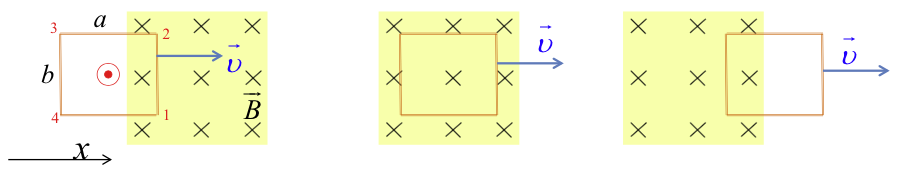
\includegraphics[width=0.88\textwidth]{./images/schematics/circuit_moving_through_magnetic_field_all_3.png}
\end{center}

\begin{columns}
  \begin{column}{0.55\textwidth}
  In summary:
  {\small
    \setlength{\extrarowheight}{10pt}
    \setlength{\arraycolsep}{5pt}
    \begin{table}[H]
        \begin{tabular}{|c||c|c|}
        \hline
               & $\displaystyle \oint_{L} \vec{E} \cdot d\vec{\ell}$ & $\displaystyle \frac{d\Phi_{M}}{dt}$\\
        \hline
          left   &  uBb &  -uBb \\
          centre & 0    &  0   \\
          right  &  -uBb & uBb \\
        \hline
        \end{tabular}
    \end{table}
  }
  \end{column}
  \begin{column}{0.45\textwidth}
     So, indeed, in all cases:
     \begin{equation*}
       \mathcal{E} = \oint_{L} \vec{E} \cdot d\vec{\ell} = - \frac{d\Phi_{M}}{dt}
     \end{equation*}
  \end{column}
\end{columns}

\end{frame}

%
%
%

\begin{frame}{Lecture \summarizedlecture revision (Faraday's observations)}

In 1831 Michael Faraday reported on a series of experiments.\\
\vspace{0.2cm}

A current flows in a wire loop when:
\vspace{0.1cm}
\begin{enumerate}[(a)]
{\small
  \item the loop is pulled through a magnetic field,
  \item the loop is at rest but the magnet moves in the opposite direction, and
  \item both the loop and the magnet are at rest but the strength of the magnetic field is varied
}
\end{enumerate}

\begin{center}
  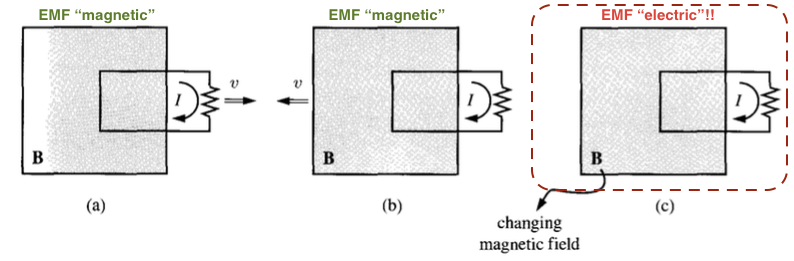
\includegraphics[width=0.80\textwidth]{./images/schematics/faraday_law_schematic_with_notes.png}
\end{center}
This led Faraday to realize that:
\begin{center}
{\bf A time-varying magnetic field induces an electic field}
\end{center}

\end{frame}

%
%
%

\begin{frame}{Lecture \summarizedlecture revision (Faraday's law / Lenz's law)}

In all cases the {\bf motional EMF} is directly related
to the {\bf change of the magnetic flux $\Phi_{M}$ though the circuit}:\\

\vspace{0.1cm}

\begin{columns} [T]
  \begin{column}{0.25\textwidth}
    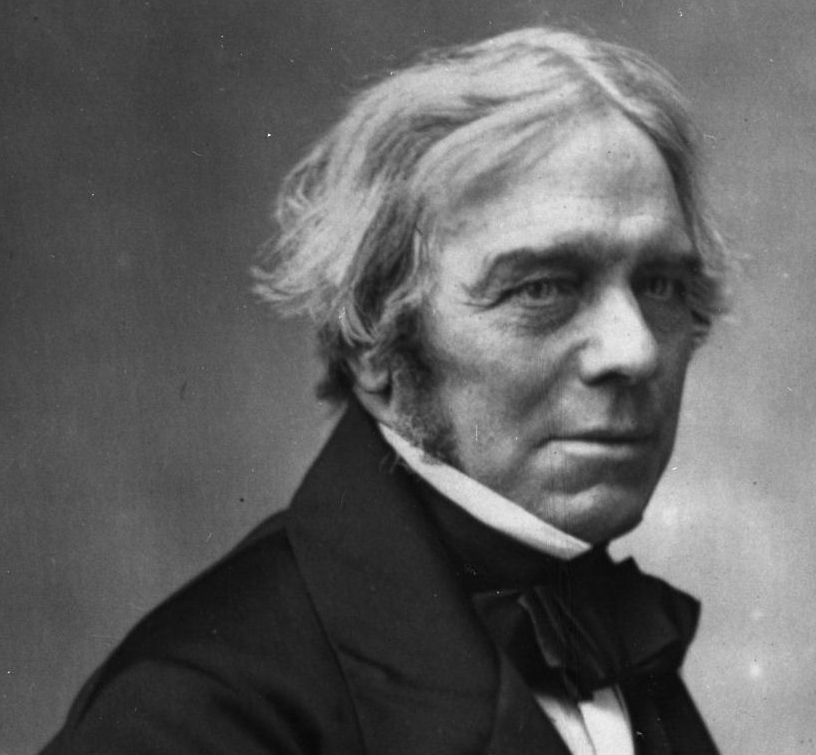
\includegraphics[width=0.98\textwidth]{./images/people/faraday.png}\\
    {\tiny Michael Faraday (1791 - 1867).}
  \end{column}
  \begin{column}{0.75\textwidth}
   \begin{center}
    \begin{equation*}
      \mathcal{E} = \oint_{L} \vec{E} \cdot d\vec{\ell} = - \frac{d\Phi_{M}}{dt}
    \end{equation*}
    \vspace{0.2cm}
    This is the so-called {\bf Faraday's law}.
   \end{center}
  \end{column}
\end{columns}

\vspace{0.1cm}

\begin{columns}
  \begin{column}{0.75\textwidth}
  {\scriptsize
    Lenz' law (1845): The EMF induced by a changing flux has a polarity
    such that the current flowing gives rise to a flux which opposes the change of flux.\\
    \vspace{0.1cm}
    The minus sign is a consequence of the {\bf conservation of energy} and
    of {\bf Newton's 3rd law} of motion: Induction is a an ``inertial reaction''.
    The system develops a current which tries to maintain the flux constant.\\
  }
  \end{column}
  \begin{column}{0.25\textwidth}
    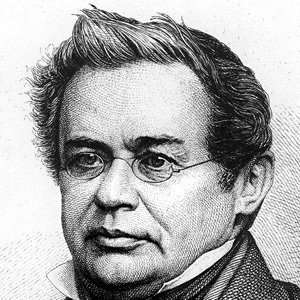
\includegraphics[width=0.83\textwidth]{./images/people/lenz.jpg}\\
    {\tiny Heinrich Lenz (1804 - 1865).}
  \end{column}
\end{columns}

\end{frame}

%
%
%

\begin{frame}{Lecture \summarizedlecture revision (Maxwell correction in Ampere's law)}

We also studied a case where Ampere's law led to paradoxical results.\\

\vspace{0.2cm}

We also saw that Ampere's law (as we knew it) was inconsistent with
the continuity equation (which expresses the local conservation of charge).\\

\vspace{0.2cm}

The problem of course was that we took a law from magnetostatics and
applied it in a different context (electrodynamics) where it is no longer valid.

\vspace{0.2cm}

Maxwell realised that all it takes to fix Ampere's law is to do the following substitution:
\begin{equation*}
  \vec{j} \rightarrow
  \vec{j} + \epsilon_0 \frac{\partial \vec{E}}{\partial t}
\end{equation*}

The term $\displaystyle \epsilon_0 \frac{\partial \vec{E}}{\partial t}$
is called {\bf displacement current}.

\end{frame}

%
%
%

\begin{frame}{Lecture \summarizedlecture revision (Maxwell's eqs for the dynamic case)}

Compared with what we had seen in the study of electrostatics and magnetostatics,
the study of time-dependent fields (electrodynamics) brought the following complication:\\

\vspace{0.1cm}

\begin{itemize}
   \item {\bf Electric fields are produced} not only by electric charges,
             but also {\bf by changing magnetic fields!}
     \begin{equation*}
        \vec{\nabla} \times \vec{E} = {\color{red} - \frac{\partial \vec{B}}{\partial t}}
     \end{equation*}

   \item {\bf Magnetic fields are produced} not only by electric currents,
             but also {\bf by changing electric fields!}
     \begin{equation*}
         \vec{\nabla} \times \vec{B} = \mu_{0} \Big( \vec{j} + {\color{red} \epsilon_0 \frac{\partial \vec{E}}{\partial t} } \Big)
     \end{equation*}
\end{itemize}

{\small
The full list of Maxwell equations for the static and dynamic cases in vacuum is shown on the next slide.
Notice that all 4 equations are coupled in the dynamic case.\\
}

\end{frame}

%
%
%

\begin{frame}{Lecture \summarizedlecture revision (Maxwell's eqs. for the dynamic case)}

{\small

\begin{center}
{
  \begin{table}[H]
    \begin{tabular}{|l|c|c|}
      \hline
        \multicolumn{3}{|l|} {
          {\color{magenta}
           {\bf Static case (in vacuum)}
          }
        }\\
      \hline
      {\bf Gauss's law} &
        $\displaystyle \oint \vec{E} d\vec{S} = \frac{1}{\epsilon_0} \int \rho d\tau$ &
        $\displaystyle \vec{\nabla} \cdot \vec{E} = \frac{\rho}{\epsilon_0}$ \\

      {\bf Circuital law} &
        $\displaystyle \oint \vec{E} d\vec{\ell} = 0$ &
        $\displaystyle \vec{\nabla} \times \vec{E} = 0$ \\

      no magn. monopoles' &
        $\displaystyle  \oint \vec{B} d\vec{S} = 0$ &
        $\displaystyle  \vec{\nabla} \cdot \vec{B} = 0$ \\

      {\bf Ampere's law} &
        $\displaystyle \oint \vec{B} d\vec{\ell} = \mu_{0} \int \vec{j} d\vec{S}$ &
        $\displaystyle \vec{\nabla} \times \vec{B} = \mu_{0} \vec{j}$ \\
      \hline
    \end{tabular}
  \end{table}
}
\end{center}


\begin{center}
{
  \begin{table}[H]
    \begin{tabular}{|l|c|c|}
      \hline
        \multicolumn{3}{|l|} {
          {\color{magenta}
           {\bf Generalization of above for the dynamic case (in vacuum)}
          }
        }\\
      \hline
      {\bf Gauss's law} &
        $\displaystyle \oint \vec{E} d\vec{S} = \frac{1}{\epsilon_0} \int \rho d\tau$ &
        $\displaystyle \vec{\nabla} \cdot \vec{E} = \frac{\rho}{\epsilon_0}$ \\

      {\bf Circuital law} &
        $\displaystyle \oint \vec{E} d\vec{\ell} =  -\frac{\partial}{\partial t} \int \vec{B} d\vec{S}$ &
        $\displaystyle \vec{\nabla} \times \vec{E} = -  \frac{\partial \vec{B}}{\partial t}$ \\

      no magn. monopoles &
        $\displaystyle  \oint \vec{B} d\vec{S} = 0$ &
        $\displaystyle  \vec{\nabla} \cdot \vec{B} = 0$ \\

      {\bf Ampere's law} &
        $\displaystyle \oint \vec{B} d\vec{\ell} = \mu_{0} \int \Big( \vec{j} + \epsilon_0 \frac{\partial \vec{E}}{\partial t}\Big) d\vec{S}$ &
        $\displaystyle \vec{\nabla} \times \vec{B} = \mu_{0} \Big( \vec{j} + \epsilon_0 \frac{\partial \vec{E}}{\partial t}\Big)$ \\
      \hline
    \end{tabular}
  \end{table}
}
\end{center}

}
\end{frame}



%
%
%

\begin{frame}{Lecture \summarizedlecture - \lecturesummarytitle}

Compared with what we had seen in the study of electrostatics and magnetostatics,
the study of time-dependent fields (electrodynamics) brought the following complication:\\

\vspace{0.1cm}

\begin{itemize}
   \item {\bf Electric fields are produced} not only by electric charges,
             but also {\bf by changing magnetic fields!}
     \begin{equation*}
        \vec{\nabla} \times \vec{E} = {\color{red} - \frac{\partial \vec{B}}{\partial t}}
     \end{equation*}

   \item {\bf Magnetic fields are produced} not only by electric currents,
             but also {\bf by changing electric fields!}
     \begin{equation*}
         \vec{\nabla} \times \vec{B} = \mu_{0} \Big( \vec{j} + {\color{red} \epsilon_0 \frac{\partial \vec{E}}{\partial t} } \Big)
     \end{equation*}
\end{itemize}

{\small
The full list of Maxwell equations for the static and dynamic cases in vacuum is shown on the next slide.
Notice that whereas the 2 equations involving $\vec{E}$ and the 2 equations involving $\vec{B}$ were decoupled in the static case,
all 4 equations are coupled in the dynamic case.\\
}

\end{frame}


%
%
%

\begin{frame}{Maxwell's equations for the static and dynamic cases}

{\small

\begin{center}
{
  \begin{table}[H]
    \begin{tabular}{|l|c|c|}
      \hline
        \multicolumn{3}{|l|} {
          {\color{magenta}
           {\bf Static case (in vacuum)}
          }
        }\\
      \hline
      {\bf Gauss's law} &
        $\displaystyle \oint \vec{E} d\vec{S} = \frac{1}{\epsilon_0} \int \rho d\tau$ &
        $\displaystyle \vec{\nabla} \cdot \vec{E} = \frac{\rho}{\epsilon_0}$ \\

      {\bf Circuital law} &
        $\displaystyle \oint \vec{E} d\vec{\ell} = 0$ &
        $\displaystyle \vec{\nabla} \times \vec{E} = 0$ \\

      no magn. monopoles' &
        $\displaystyle  \oint \vec{B} d\vec{S} = 0$ &
        $\displaystyle  \vec{\nabla} \cdot \vec{B} = 0$ \\

      {\bf Ampere's law} &
        $\displaystyle \oint \vec{B} d\vec{\ell} = \mu_{0} \int \vec{j} d\vec{S}$ &
        $\displaystyle \vec{\nabla} \times \vec{B} = \mu_{0} \vec{j}$ \\
      \hline
    \end{tabular}
  \end{table}
}
\end{center}


\begin{center}
{
  \begin{table}[H]
    \begin{tabular}{|l|c|c|}
      \hline
        \multicolumn{3}{|l|} {
          {\color{magenta}
           {\bf Generalization of above for the dynamic case (in vacuum)}
          }
        }\\
      \hline
      {\bf Gauss's law} &
        $\displaystyle \oint \vec{E} d\vec{S} = \frac{1}{\epsilon_0} \int \rho d\tau$ &
        $\displaystyle \vec{\nabla} \cdot \vec{E} = \frac{\rho}{\epsilon_0}$ \\

      {\bf Circuital law} &
        $\displaystyle \oint \vec{E} d\vec{\ell} =  -\frac{\partial}{\partial t} \int \vec{B} d\vec{S}$ &
        $\displaystyle \vec{\nabla} \times \vec{E} = -  \frac{\partial \vec{B}}{\partial t}$ \\

      no magn. monopoles &
        $\displaystyle  \oint \vec{B} d\vec{S} = 0$ &
        $\displaystyle  \vec{\nabla} \cdot \vec{B} = 0$ \\

      {\bf Ampere's law} &
        $\displaystyle \oint \vec{B} d\vec{\ell} = \mu_{0} \int \Big( \vec{j} + \epsilon_0 \frac{\partial \vec{E}}{\partial t}\Big) d\vec{S}$ &
        $\displaystyle \vec{\nabla} \times \vec{B} = \mu_{0} \Big( \vec{j} + \epsilon_0 \frac{\partial \vec{E}}{\partial t}\Big)$ \\
      \hline
    \end{tabular}
  \end{table}
}
\end{center}

}
\end{frame}


%
% Plan for the next lecture
%

\begin{frame}{At the next lecture (Lecture \nextlecture)}

\begin{itemize}
  \item We will study the solutions of the time-dependent Maxwell equations in vaccum
            away from sources ($\rho = 0$, $\vec{j} = \vec{0}$)
  \vspace{0.3cm}
  \item {\bf Light}!
\end{itemize}

\vspace{0.3cm}

\begin{center}
   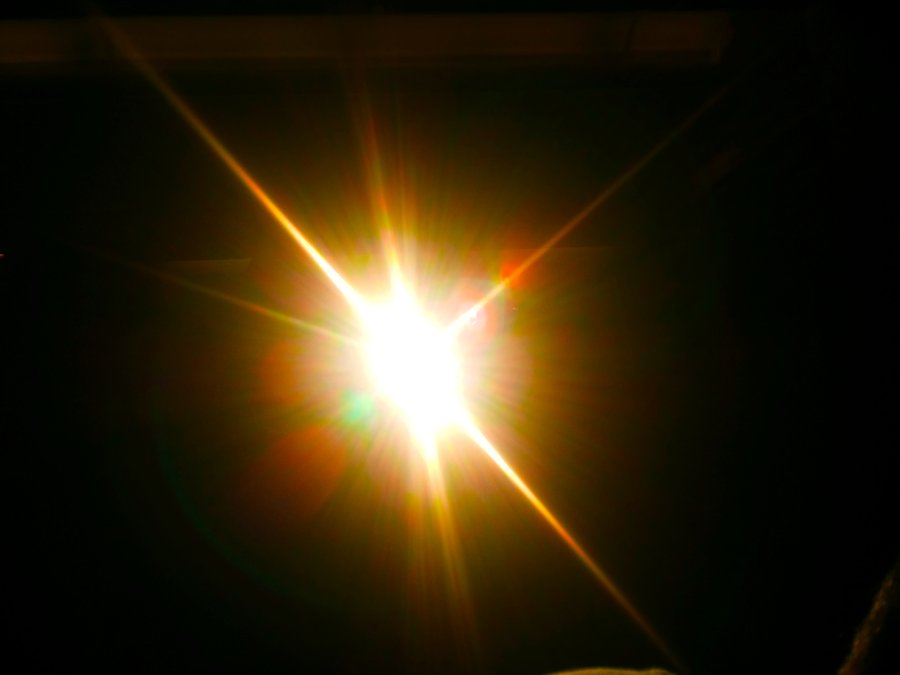
\includegraphics[width=0.55\textwidth]{./images/photos/beam_of_light.jpg}\\
\end{center}

\end{frame}

% ------------------------------------------------------------------------------
% ------------------------------------------------------------------------------
